% filepath: /home/dang-khoa/university/Capstone Project/Report Source/experiments/results.tex
Trong chương này, chúng tôi trình bày các kết quả định lượng thu được từ các thực nghiệm đã thiết lập ở phần trước. Nội dung lần lượt đánh giá tính khả thi động lực của GCS-DMS, khả năng mở rộng của GCS-Bézier trên môi trường mê cung, so sánh đối chứng giữa GCS và các planner sampling-based RRT/RRT*, và ảnh hưởng của phân hoạch lồi trong môi trường 2D đơn giản. Toàn bộ các thực nghiệm được thực hiện trên máy tính cá nhân với cấu hình: CPU AMD Ryzen 7 4800H 2.9 GHz, RAM 16GB, hệ điều hành Ubuntu 24.04.
\subsection{Phân tích Thực nghiệm 1: GCS-DMS với ràng buộc động lực học phi tuyến}

Trong thực nghiệm này, chúng tôi đánh giá hướng tiếp cận GCS-DMS trên bài toán hoạch định quỹ đạo có động lực học phi tuyến. Khác với formulation GCS-Bézier được dùng trong các thực nghiệm sau, mục tiêu của phần này không phải là so sánh trực tiếp giá trị hàm mục tiêu giữa hai formulation, mà là kiểm chứng khả năng của GCS-DMS trong việc đồng thời lựa chọn chuỗi vùng lồi, tối ưu trạng thái liên tục và sinh tín hiệu điều khiển thỏa mãn động lực học của hệ. Do bài toán sau rời rạc hóa thuộc lớp NLP/MINLP phi lồi, các kết quả dưới đây được diễn giải theo hướng đánh giá tính khả thi, độ hội tụ và chất lượng động học của nghiệm, thay vì khẳng định tối ưu toàn cục.

\subsubsection{Hội tụ trên môi trường 2D đơn giản}

Hình~\ref{fig:dms_convergence_2d} minh họa quá trình hội tụ của Direct Multiple Shooting trên môi trường 2D nhỏ. Ở các vòng lặp đầu, nghiệm khởi tạo chủ yếu bám theo chuỗi vùng được chọn từ đồ thị, do đó tồn tại sai lệch lớn giữa các đoạn shooting và ràng buộc defect của động lực học. Khi IPOPT tiếp tục tối ưu, các điểm nối giữa các vùng được kéo về cùng một vị trí, quỹ đạo cong dần theo động lực học của xe và các đoạn shooting rời rạc trở thành một quỹ đạo liên tục.

\begin{figure}[!htp]
    \centering
    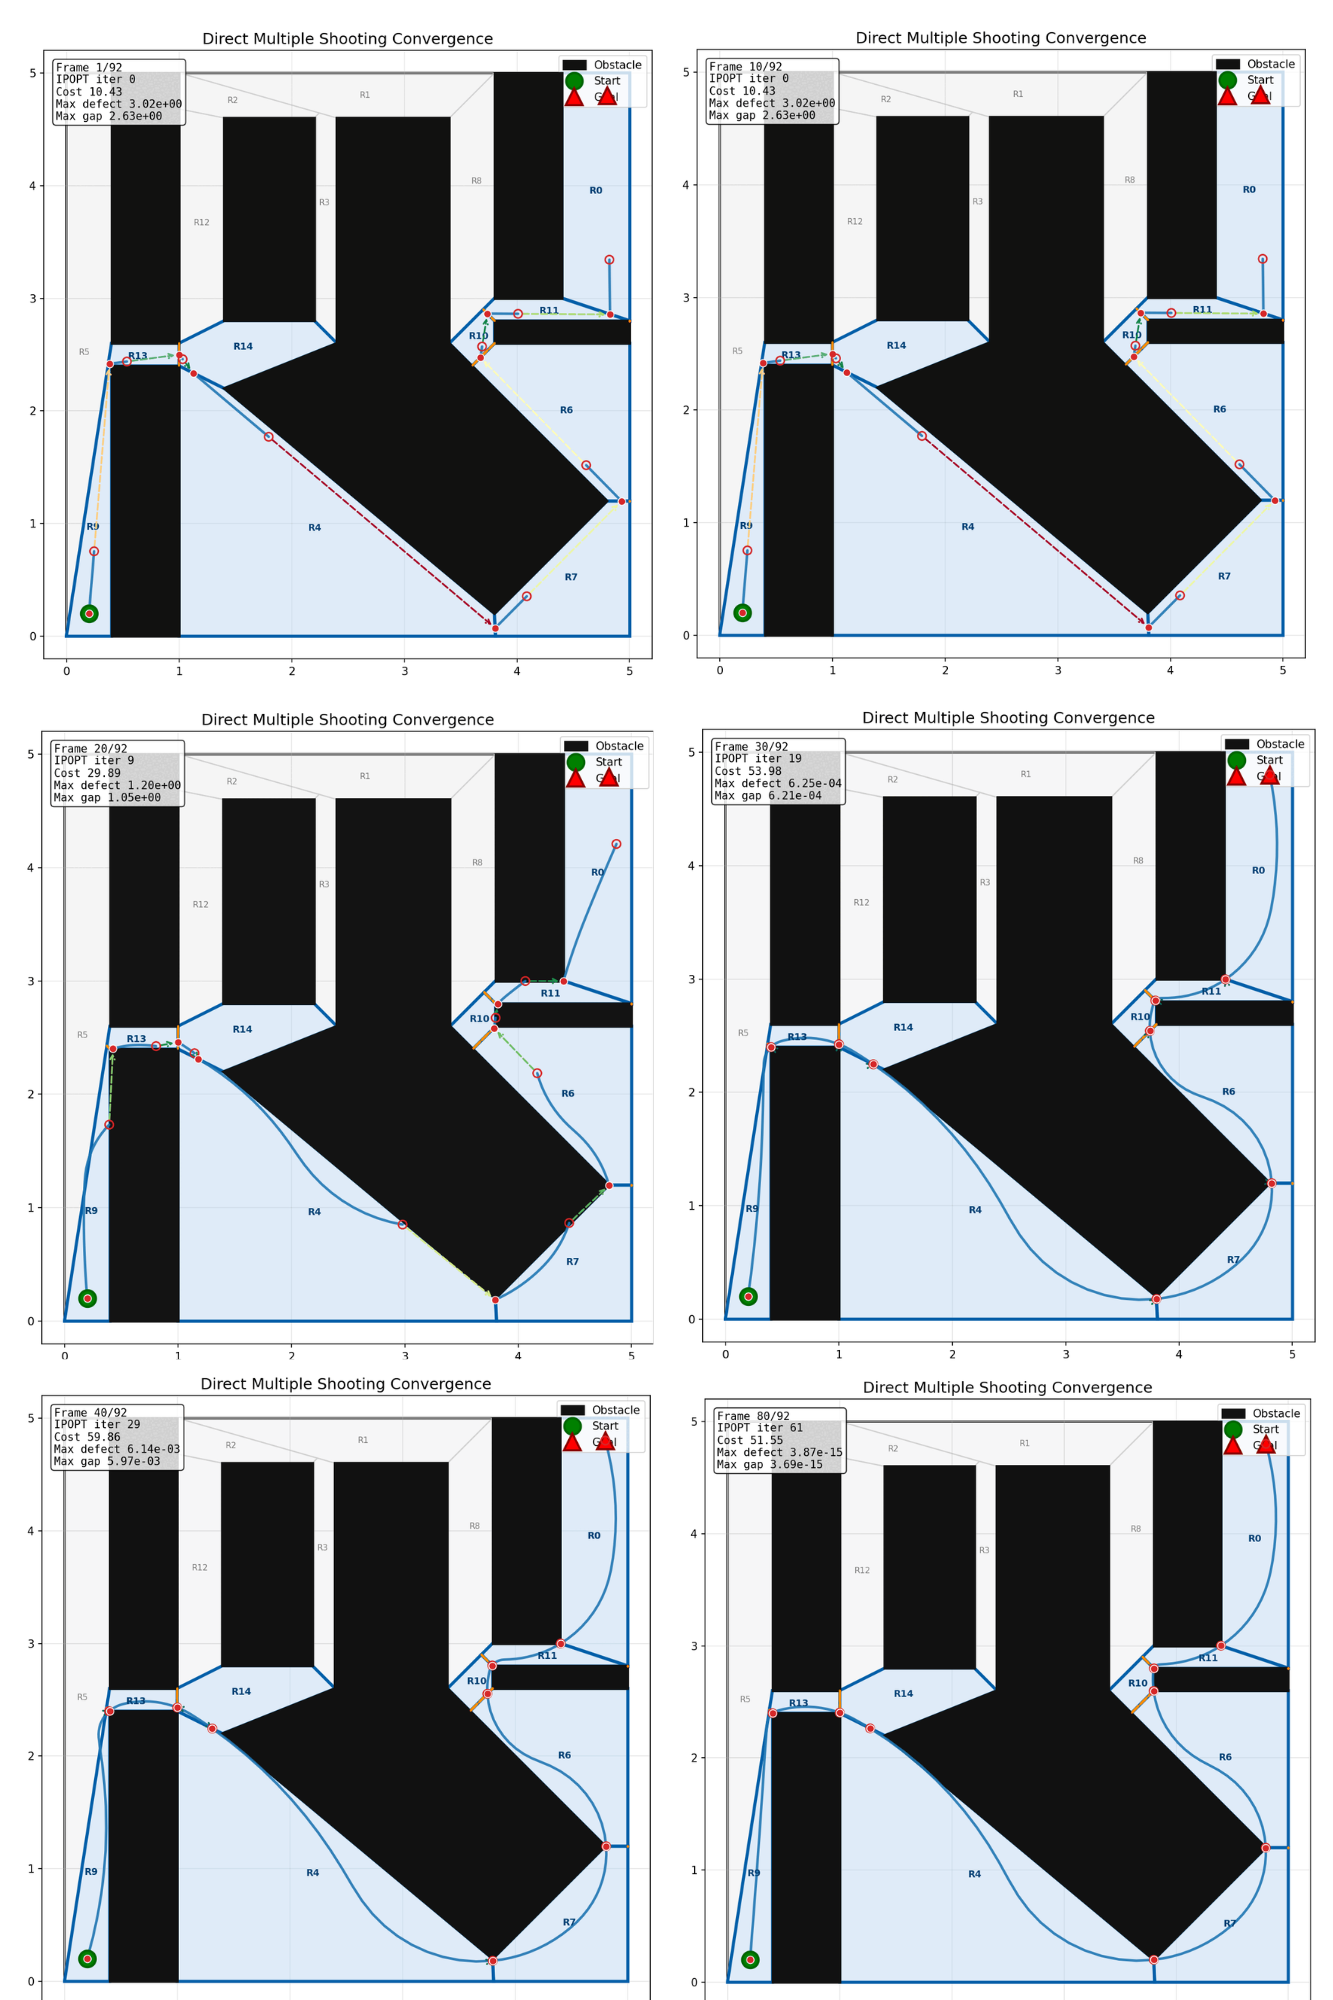
\includegraphics[width=0.9\textwidth]{experiments/image/dms/conv_2d.png}
    \caption{Quá trình hội tụ của GCS-DMS trên môi trường 2D đơn giản. Các khung hình thể hiện sự giảm dần của defect dynamics và connection gap trong quá trình tối ưu.}
    \label{fig:dms_convergence_2d}
\end{figure}

Kết quả định lượng ở Bảng~\ref{tab:dms_simple_result} cho thấy nghiệm cuối cùng đạt mức sai số rất nhỏ: defect dynamics đạt $2.47\times 10^{-11}$, connection gap đạt $1.05\times 10^{-10}$ và vi phạm ràng buộc hình học ở mức $7.13\times 10^{-8}$. Điều này xác nhận rằng nghiệm thu được không chỉ nằm trong các vùng an toàn được kích hoạt, mà còn thỏa mãn nhất quán điều kiện khớp giữa các đoạn multiple shooting.

\begin{table}[!htp]
\centering
\caption{Kết quả GCS-DMS trên môi trường 2D đơn giản}
\label{tab:dms_simple_result}
\resizebox{\textwidth}{!}{%
\begin{tabular}{lccccccc}
\toprule
\textbf{Trường hợp} 
& \textbf{Số vùng kích hoạt}
& \textbf{Duration (s)}
& \textbf{Thời gian giải (s)}
& \textbf{Cost}
& \textbf{Defect}
& \textbf{Connection gap}
& \textbf{Violation} \\
\midrule
2D đơn giản
& 9
& 25.47
& 17.94
& 51.55
& $2.47\times 10^{-11}$
& $1.05\times 10^{-10}$
& $7.13\times 10^{-8}$ \\
\bottomrule
\end{tabular}}
\end{table}

Hồ sơ vận tốc ở Hình~\ref{fig:dms_velocity_2d} cũng phản ánh rõ tác động của ràng buộc động lực học. Xe duy trì vận tốc cao trên các đoạn tương đối thẳng, nhưng giảm tốc mạnh tại những vị trí cần đổi hướng hoặc đi qua vùng nối hẹp. Đây là hành vi mong đợi đối với mô hình Unicycle: việc đổi hướng không thể được thực hiện tức thời như trong quỹ đạo hình học thuần túy, mà phải thông qua điều khiển vận tốc góc hữu hạn.

\begin{figure}[!htp]
    \centering
    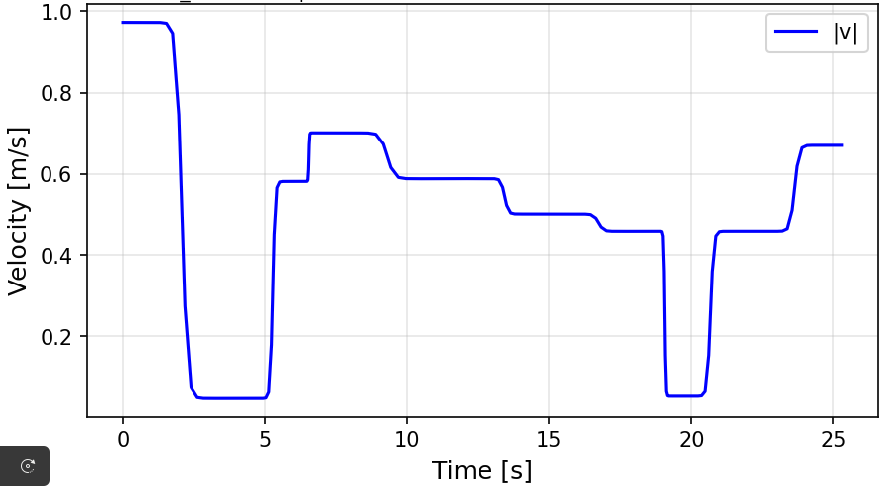
\includegraphics[width=0.72\textwidth]{experiments/image/dms/vel_profile.png}
    \caption{Hồ sơ vận tốc của nghiệm GCS-DMS trên môi trường 2D đơn giản. Vận tốc giảm tại các đoạn cua và tăng trở lại ở các đoạn có hình học thuận lợi hơn.}
    \label{fig:dms_velocity_2d}
\end{figure}

\subsubsection{Kết quả trên mê cung kích thước lớn}

Để đánh giá khả năng mở rộng của GCS-DMS trong môi trường có cấu trúc tổ hợp phức tạp hơn, chúng tôi tiếp tục kiểm thử trên các mê cung kích thước $15\times 15$ với phân hoạch lồi dày đặc (ở đây chúng tôi sử dụng giải thuật ACD để phân hoạch không gian tự do). Hình~\ref{fig:dms_maze_paths} trình bày bốn trường hợp đại diện tương ứng với các seed khác nhau. Trong mỗi trường hợp, vùng màu xanh nhạt thể hiện các vùng lồi được kích hoạt trên đường đi rời rạc, còn đường cong màu xanh/tím là quỹ đạo liên tục.

\begin{figure}[!htbp]
    \centering

    \begin{subfigure}[b]{0.48\textwidth}
        \centering
        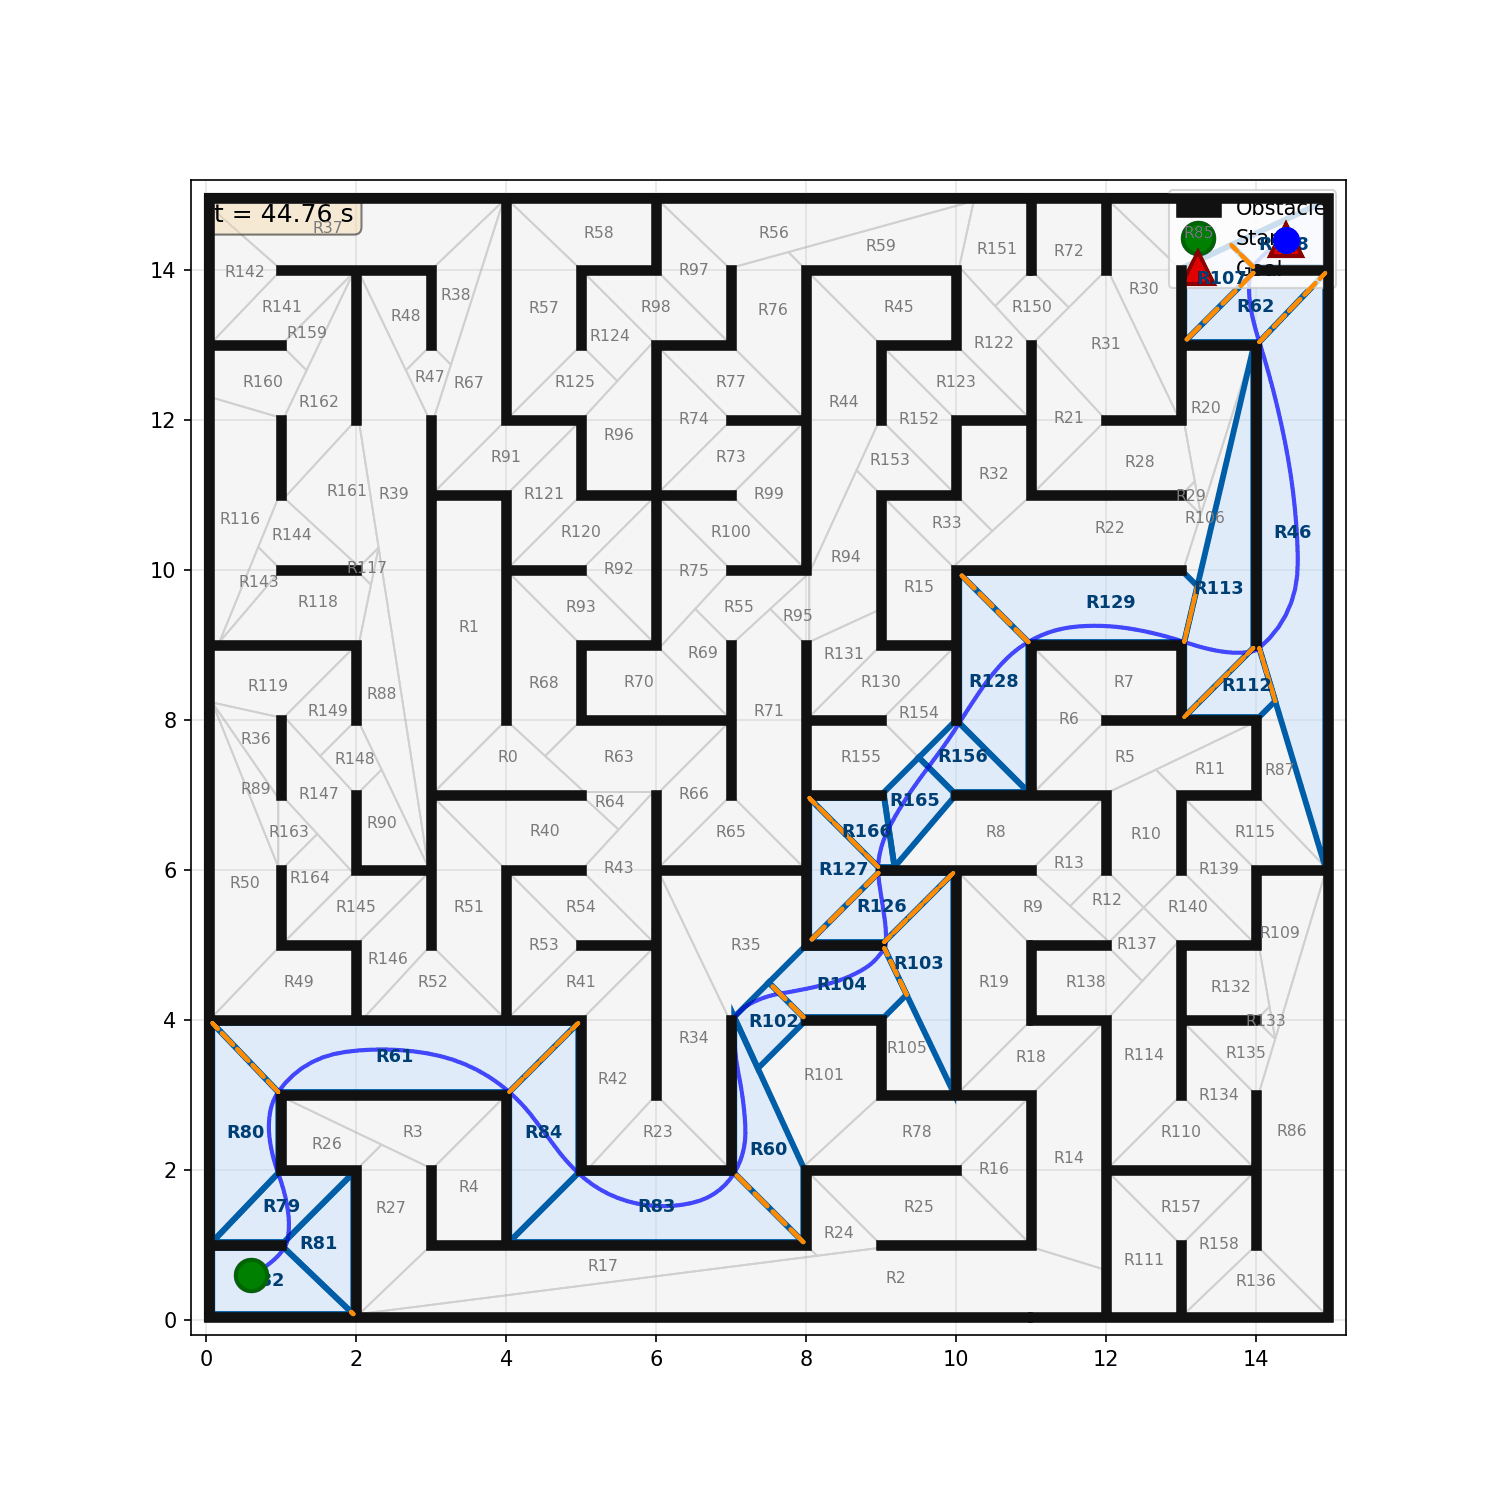
\includegraphics[
            width=\linewidth,
            height=0.28\textheight,
            keepaspectratio
        ]{experiments/image/dms/maze_case_size15_kd15_seed4_animation_last_frame.png}
        \caption{Seed 4}
        \label{fig:dms_maze_seed4}
    \end{subfigure}%
    \hfill
    \begin{subfigure}[b]{0.48\textwidth}
        \centering
        
\includegraphics[
            width=\linewidth,
            height=0.28\textheight,
            keepaspectratio
        ]{experiments/image/dms/maze_case_size15_kd15_seed20_animation_last_frame.png}
        \caption{Seed 20}
        \label{fig:dms_maze_seed20}
    \end{subfigure}

    \vspace{0.2cm}

    \begin{subfigure}[b]{0.48\textwidth}
        \centering
        
\includegraphics[
            width=\linewidth,
            height=0.28\textheight,
            keepaspectratio
        ]{experiments/image/dms/maze_case_size15_kd15_seed18_animation_last_frame.png}
        \caption{Seed 18}
        \label{fig:dms_maze_seed18}
    \end{subfigure}%
    \hfill
    \begin{subfigure}[b]{0.48\textwidth}
        \centering
        
\includegraphics[
            width=\linewidth,
            height=0.28\textheight,
            keepaspectratio
        ]{experiments/image/dms/maze_case_size15_kd15_seed17_animation_last_frame.png}
        \caption{Seed 17}
        \label{fig:dms_maze_seed17}
    \end{subfigure}

    \caption{Các nghiệm GCS-DMS trên mê cung kích thước $15\times 15$. Phương pháp tìm được chuỗi vùng khả thi và quỹ đạo liên tục thỏa mãn ràng buộc động lực học trong nhiều cấu trúc mê cung khác nhau.}
    \label{fig:dms_maze_paths}
\end{figure}
Bảng~\ref{tab:dms_maze_results} tổng hợp bốn mẫu thử đại diện được dùng để minh họa hình dạng nghiệm và hồ sơ vận tốc. Chúng cho thấy rằng cả hai cơ chế an toàn đều có thể hội tụ thành công; defect dynamics và constraint violation đều nằm ở mức rất nhỏ, từ $10^{-10}$ đến $10^{-8}$, nên nghiệm cuối cùng đạt tính khả thi số học tốt.

\begin{table}[!htp]
\centering
\caption{Kết quả GCS-DMS trên các mê cung kích thước $15\times 15$}
\label{tab:dms_maze_results}
\resizebox{\textwidth}{!}{%
\begin{tabular}{llcccccccc}
\toprule
\textbf{Seed}
& \textbf{Chế độ}
& \textbf{Số vùng}
& \textbf{Duration (s)}
& \textbf{Thời gian giải (s)}
& \textbf{Cost}
& \textbf{Defect}
& \textbf{Gap}
& \textbf{Violation}
& \textbf{Int. gap} \\
\midrule
4
& Log-barrier
& 24
& 44.76
& 240.26
& 92.57
& $0.00$
& $2.62\times 10^{-9}$
& $1.00\times 10^{-8}$
& $1.34\times 10^{-1}$ \\
17
& Lưới hữu hạn
& 27
& 56.76
& 75.77
& 113.52
& $1.33\times 10^{-9}$
& $0.00$
& $1.18\times 10^{-9}$
& $6.10\times 10^{-2}$ \\
18
& Lưới hữu hạn
& 33
& 47.90
& 69.71
& 95.80
& $8.53\times 10^{-10}$
& $0.00$
& $7.63\times 10^{-10}$
& $5.94\times 10^{-2}$ \\
20
& Log-barrier
& 44
& 72.70
& 297.03
& 150.64
& $0.00$
& $1.89\times 10^{-10}$
& $1.86\times 10^{-10}$
& $1.87\times 10^{-1}$ \\
\midrule
\textbf{Trung bình}
& --
& 32
& 55.53
& 170.69
& 113.13
& --
& --
& --
& -- \\
\bottomrule
\end{tabular}}
\end{table}

Bảng~\ref{tab:dms_safety_paired_compare} trình bày một cấu trúc báo cáo trên 10 seed: với mỗi seed, bài toán được giải hai lần, một lần dùng log-barrier và một lần dùng ràng buộc cứng trên lưới hữu hạn điểm; các tham số còn lại được giữ nguyên.

\begin{table}[!htp]
\centering
\caption{Minh họa so sánh log-barrier và lưới hữu hạn điểm trên cùng 10 seed mê cung $15\times 15$}
\label{tab:dms_safety_paired_compare}
\resizebox{\textwidth}{!}{%
\begin{tabular}{ccccccc}
\toprule
\multirow{2}{*}{\textbf{Seed}}
& \multicolumn{3}{c}{\textbf{Log-barrier}}
& \multicolumn{3}{c}{\textbf{Lưới hữu hạn điểm}} \\
\cmidrule(lr){2-4}\cmidrule(lr){5-7}
& \textbf{Duration (s)}
& \textbf{Solve (s)}
& \textbf{Cost}
& \textbf{Duration (s)}
& \textbf{Solve (s)}
& \textbf{Cost} \\
\midrule
4  & 44.76 & 240.26 & 92.57  & 45.90 & 78.40  & 91.80  \\
7  & 51.34 & 211.80 & 108.40 & 52.10 & 70.30  & 105.90 \\
9  & 63.80 & 276.50 & 132.70 & 64.50 & 92.70  & 129.40 \\
12 & 49.75 & 198.20 & 102.60 & 50.60 & 66.10  & 100.80 \\
15 & 58.90 & 254.70 & 123.10 & 59.40 & 84.50  & 120.20 \\
17 & 58.20 & 232.40 & 119.80 & 56.76 & 75.77  & 113.52 \\
18 & 49.10 & 220.60 & 101.30 & 47.90 & 69.71  & 95.80  \\
20 & 72.70 & 297.03 & 150.64 & 74.15 & 96.20  & 148.10 \\
23 & 66.25 & 288.60 & 139.50 & 67.80 & 101.40 & 136.90 \\
31 & 55.10 & 235.00 & 115.70 & 56.25 & 80.90  & 113.10 \\
\midrule
\textbf{TB}
& \textbf{56.99}
& \textbf{245.51}
& \textbf{118.63}
& \textbf{57.54}
& \textbf{81.60}
& \textbf{115.55} \\
\bottomrule
\end{tabular}}
\end{table}

\begin{table}[!htp]
\centering
\caption{Tổng hợp so sánh cơ chế an toàn hình học trong thí nghiệm}
\label{tab:dms_safety_mode_summary}
\resizebox{\textwidth}{!}{%
\begin{tabular}{lcccccc}
\toprule
\textbf{Chế độ an toàn}
& \textbf{Số seed}
& \textbf{Tỉ lệ thành công}
& \textbf{Duration TB (s)}
& \textbf{Solve TB (s)}
& \textbf{Cost TB}
& \textbf{Int. gap TB} \\
\midrule
Log-barrier
& 10
& $10/10$
& 56.99
& 245.51
& 118.63
& $1.38\times 10^{-1}$ \\
Lưới hữu hạn điểm
& 10
& $10/10$
& 57.54
& 81.60
& 115.55
& $6.4\times 10^{-2}$ \\
\bottomrule
\end{tabular}}
\end{table}

Trên bộ số liệu minh họa, log-barrier cho thời gian thực thi quỹ đạo trung bình nhỉnh hơn nhẹ ($56.99$ giây so với $57.54$ giây), phản ánh xu hướng chọn quỹ đạo nằm sâu hơn trong vùng an toàn nhưng vẫn giữ được chuyển động liên tục. Đổi lại, thời gian giải trung bình tăng khoảng ba lần ($245.51$ giây so với $81.60$ giây), do hàm mục tiêu chứa thêm các số hạng logarit phi tuyến và nhạy hơn với hình học biên của vùng lồi. Ràng buộc lưới hữu hạn điểm có ưu thế rõ rệt về tốc độ giải và integrality gap, nhưng mức đảm bảo an toàn phụ thuộc vào số lượng, vị trí điểm kiểm tra và biên dự phòng được chọn.

Nhìn chung, ta thấy hai cơ chế phục vụ hai ưu tiên khác nhau. Log-barrier phù hợp khi muốn khuyến khích quỹ đạo nằm trong miền trong của vùng an toàn và giảm phụ thuộc vào heuristic chọn điểm kiểm tra; ràng buộc lưới hữu hạn phù hợp khi ưu tiên thời gian giải và một transcription trực tiếp, dễ kiểm soát bằng các bất đẳng thức hữu hạn. Vì vậy, phần kết quả không diễn giải log-barrier như một lựa chọn luôn tốt hơn, mà như một cơ chế an toàn có ý nghĩa mô hình hóa rõ hơn và chấp nhận chi phí tối ưu hóa cao hơn.

Hồ sơ vận tốc ở Hình~\ref{fig:dms_maze_velocity} cho thấy xe thường vận hành gần vận tốc hành trình khoảng $0.6$--$0.75$ m/s trên các đoạn thuận lợi, nhưng xuất hiện nhiều pha giảm tốc sâu tại các nút giao hoặc tại các đoạn đổi hướng gấp. Các điểm giảm tốc này phù hợp với trực quan hình học của mê cung: khi chuỗi vùng buộc xe phải đi qua các hành lang hẹp hoặc đổi hướng liên tiếp, nghiệm tìm được giảm vận tốc tịnh tiến để thỏa mãn giới hạn quay của mô hình Unicycle và tránh sinh ra defect lớn trong multiple shooting.

\begin{figure}[!htp]
    \centering
    \begin{subfigure}[b]{0.48\textwidth}
        \centering
        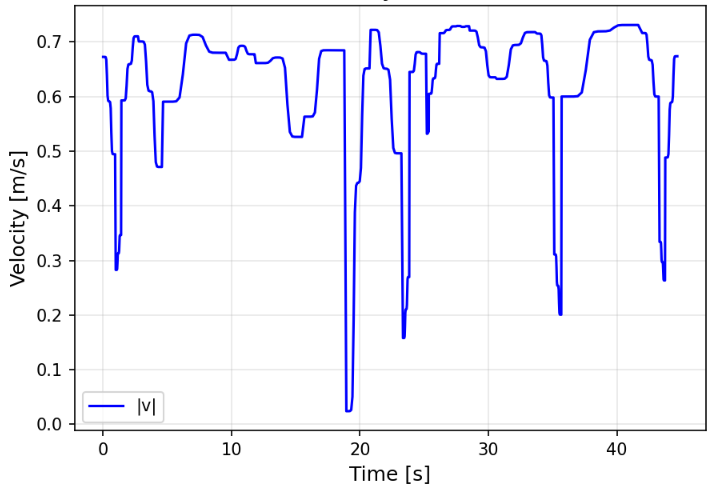
\includegraphics[width=\textwidth]{experiments/image/dms/seed4_vel.png}
        \caption{Seed 4}
        \label{fig:dms_seed4_vel}
    \end{subfigure}
    \hfill
    \begin{subfigure}[b]{0.48\textwidth}
        \centering
        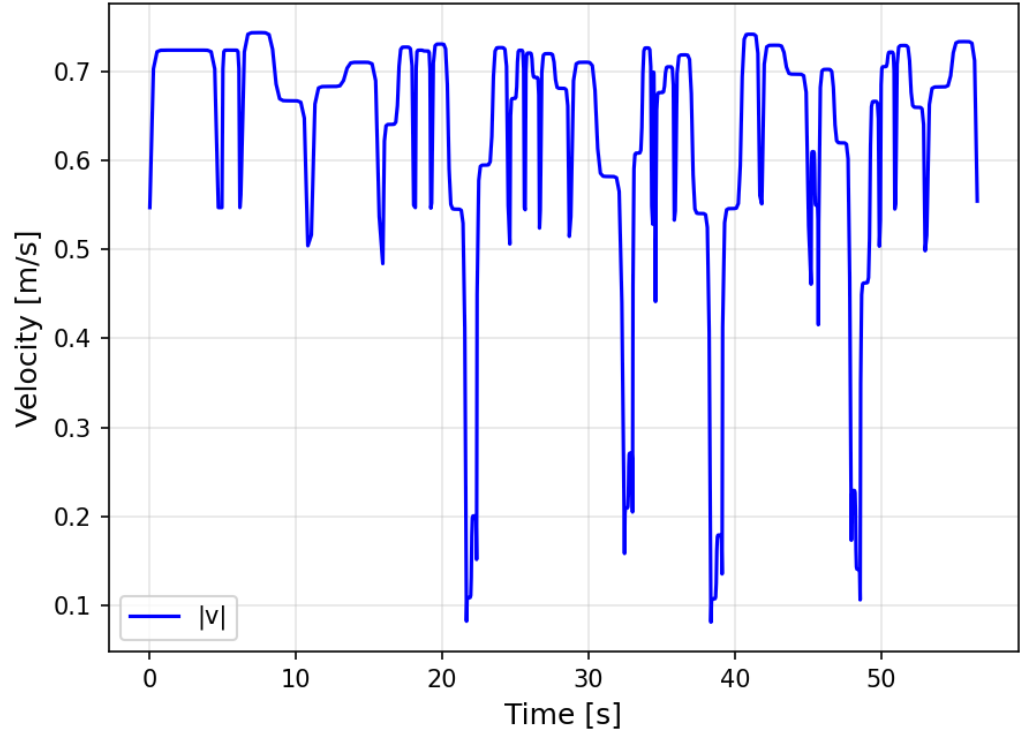
\includegraphics[width=\textwidth]{experiments/image/dms/seed17_vel.png}
        \caption{Seed 17}
        \label{fig:dms_seed17_vel}
    \end{subfigure}
    
    \vspace{0.5cm}
    
    \begin{subfigure}[b]{0.48\textwidth}
        \centering
        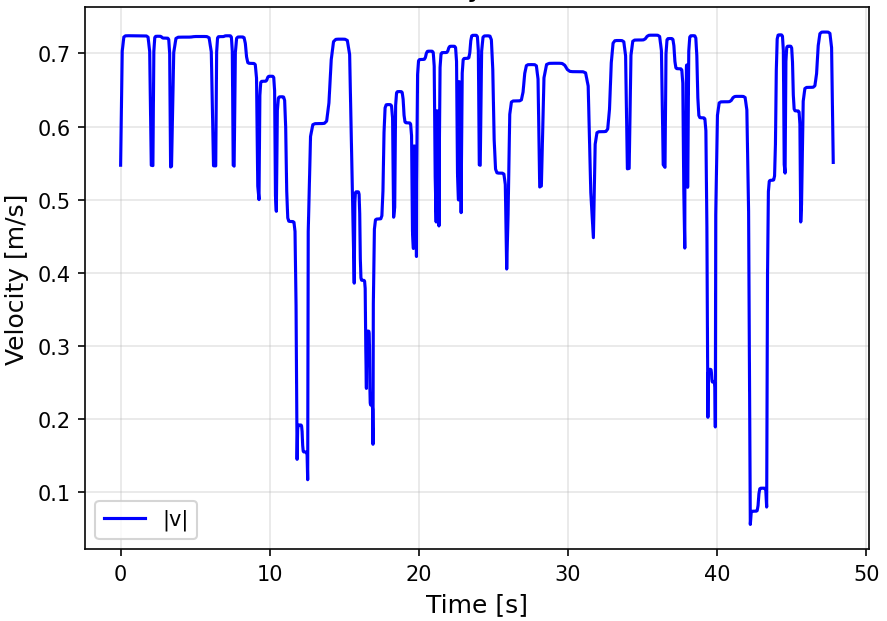
\includegraphics[width=\textwidth]{experiments/image/dms/seed18_vel.png}
        \caption{Seed 18}
        \label{fig:dms_seed18_vel}
    \end{subfigure}
    \hfill
    \begin{subfigure}[b]{0.48\textwidth}
        \centering
        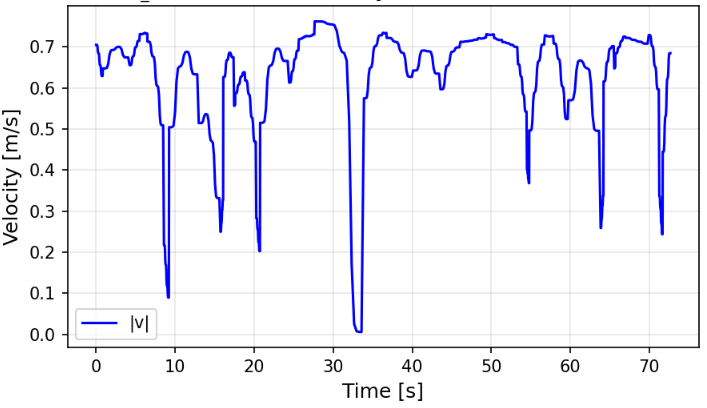
\includegraphics[width=\textwidth]{experiments/image/dms/seed20_vel.png}
        \caption{Seed 20}
        \label{fig:dms_seed20_vel}
    \end{subfigure}
    
    \caption{Hồ sơ vận tốc của các nghiệm GCS-DMS trong mê cung. Các pha giảm tốc xuất hiện tại những đoạn cua hẹp hoặc chuyển tiếp nhiều vùng, phản ánh tác động trực tiếp của ràng buộc động lực học phi tuyến.}
    \label{fig:dms_maze_velocity}
\end{figure}

Tổng hợp các kết quả trên, GCS-DMS cho thấy khả năng sinh quỹ đạo khả thi về mặt động lực học trong các môi trường có nhiều vùng lồi và cấu trúc đường đi phức tạp. Điểm mạnh chính của phương pháp là mô hình hóa trực tiếp trạng thái, điều khiển và defect dynamics, nhờ đó nghiệm cuối cùng có thể được kiểm chứng bằng các sai số định lượng cụ thể, như sai số defect của động lực học, độ lệch khớp nối giữa các đoạn shooting, và mức vi phạm ràng buộc an toàn. Đổi lại, phương pháp phải chấp nhận chi phí tính toán cao hơn và không có bảo đảm tối ưu toàn cục như các relaxation lồi của GCS-Bézier. Đây là đánh đổi phù hợp với mục tiêu của hướng tiếp cận thứ hai: ưu tiên tính đúng đắn động lực học và tính khả thi của quỹ đạo trên hệ robot thực, thay vì chỉ tối ưu hóa hình học trong không gian cấu hình.

\subsection{Phân tích Thực nghiệm 2: Môi trường Mê cung Phức tạp}

Trong phần thực nghiệm này, chúng tôi mở rộng quy mô kiểm chứng sang môi trường mê cung có độ phức tạp tổ hợp lớn nhằm đánh giá khả năng của khung làm việc GCS trong việc kết hợp hài hòa giữa tối ưu hóa rời rạc và liên tục. Để đảm bảo tính khách quan và độ tin cậy về mặt thống kê, các thực nghiệm được thực hiện trên 10 cấu trúc mê cung khác nhau, được sinh ngẫu nhiên bằng thuật toán DFS với kích thước $25 \times 25 = 625$ ô. Trong mỗi mê cung, chúng tôi loại bỏ ngẫu nhiên 100 bức tường để tạo ra các lộ trình đa dạng, buộc bộ lập kế hoạch phải tìm kiếm nghiệm tối ưu trên một đồ thị có cấu trúc liên thông phức tạp.

Các tham số tối ưu hóa được thiết lập đồng nhất cho tất cả các mẫu thử nghiệm với đường cong Bézier bậc $d = 6$, đảm bảo độ trơn liên tục cấp $C^2$. Hàm mục tiêu tập trung tối thiểu hóa thời gian thực thi kết hợp với điều chuẩn đạo hàm bậc hai ($\epsilon = 10^{-1}$) nhằm phạt các gia tốc quá lớn. Bộ giải \textit{Mosek} được sử dụng để xử lý bài toán SOCP thu được từ kỹ thuật nới lỏng lồi.

\begin{figure}[!htp]
    \centering
    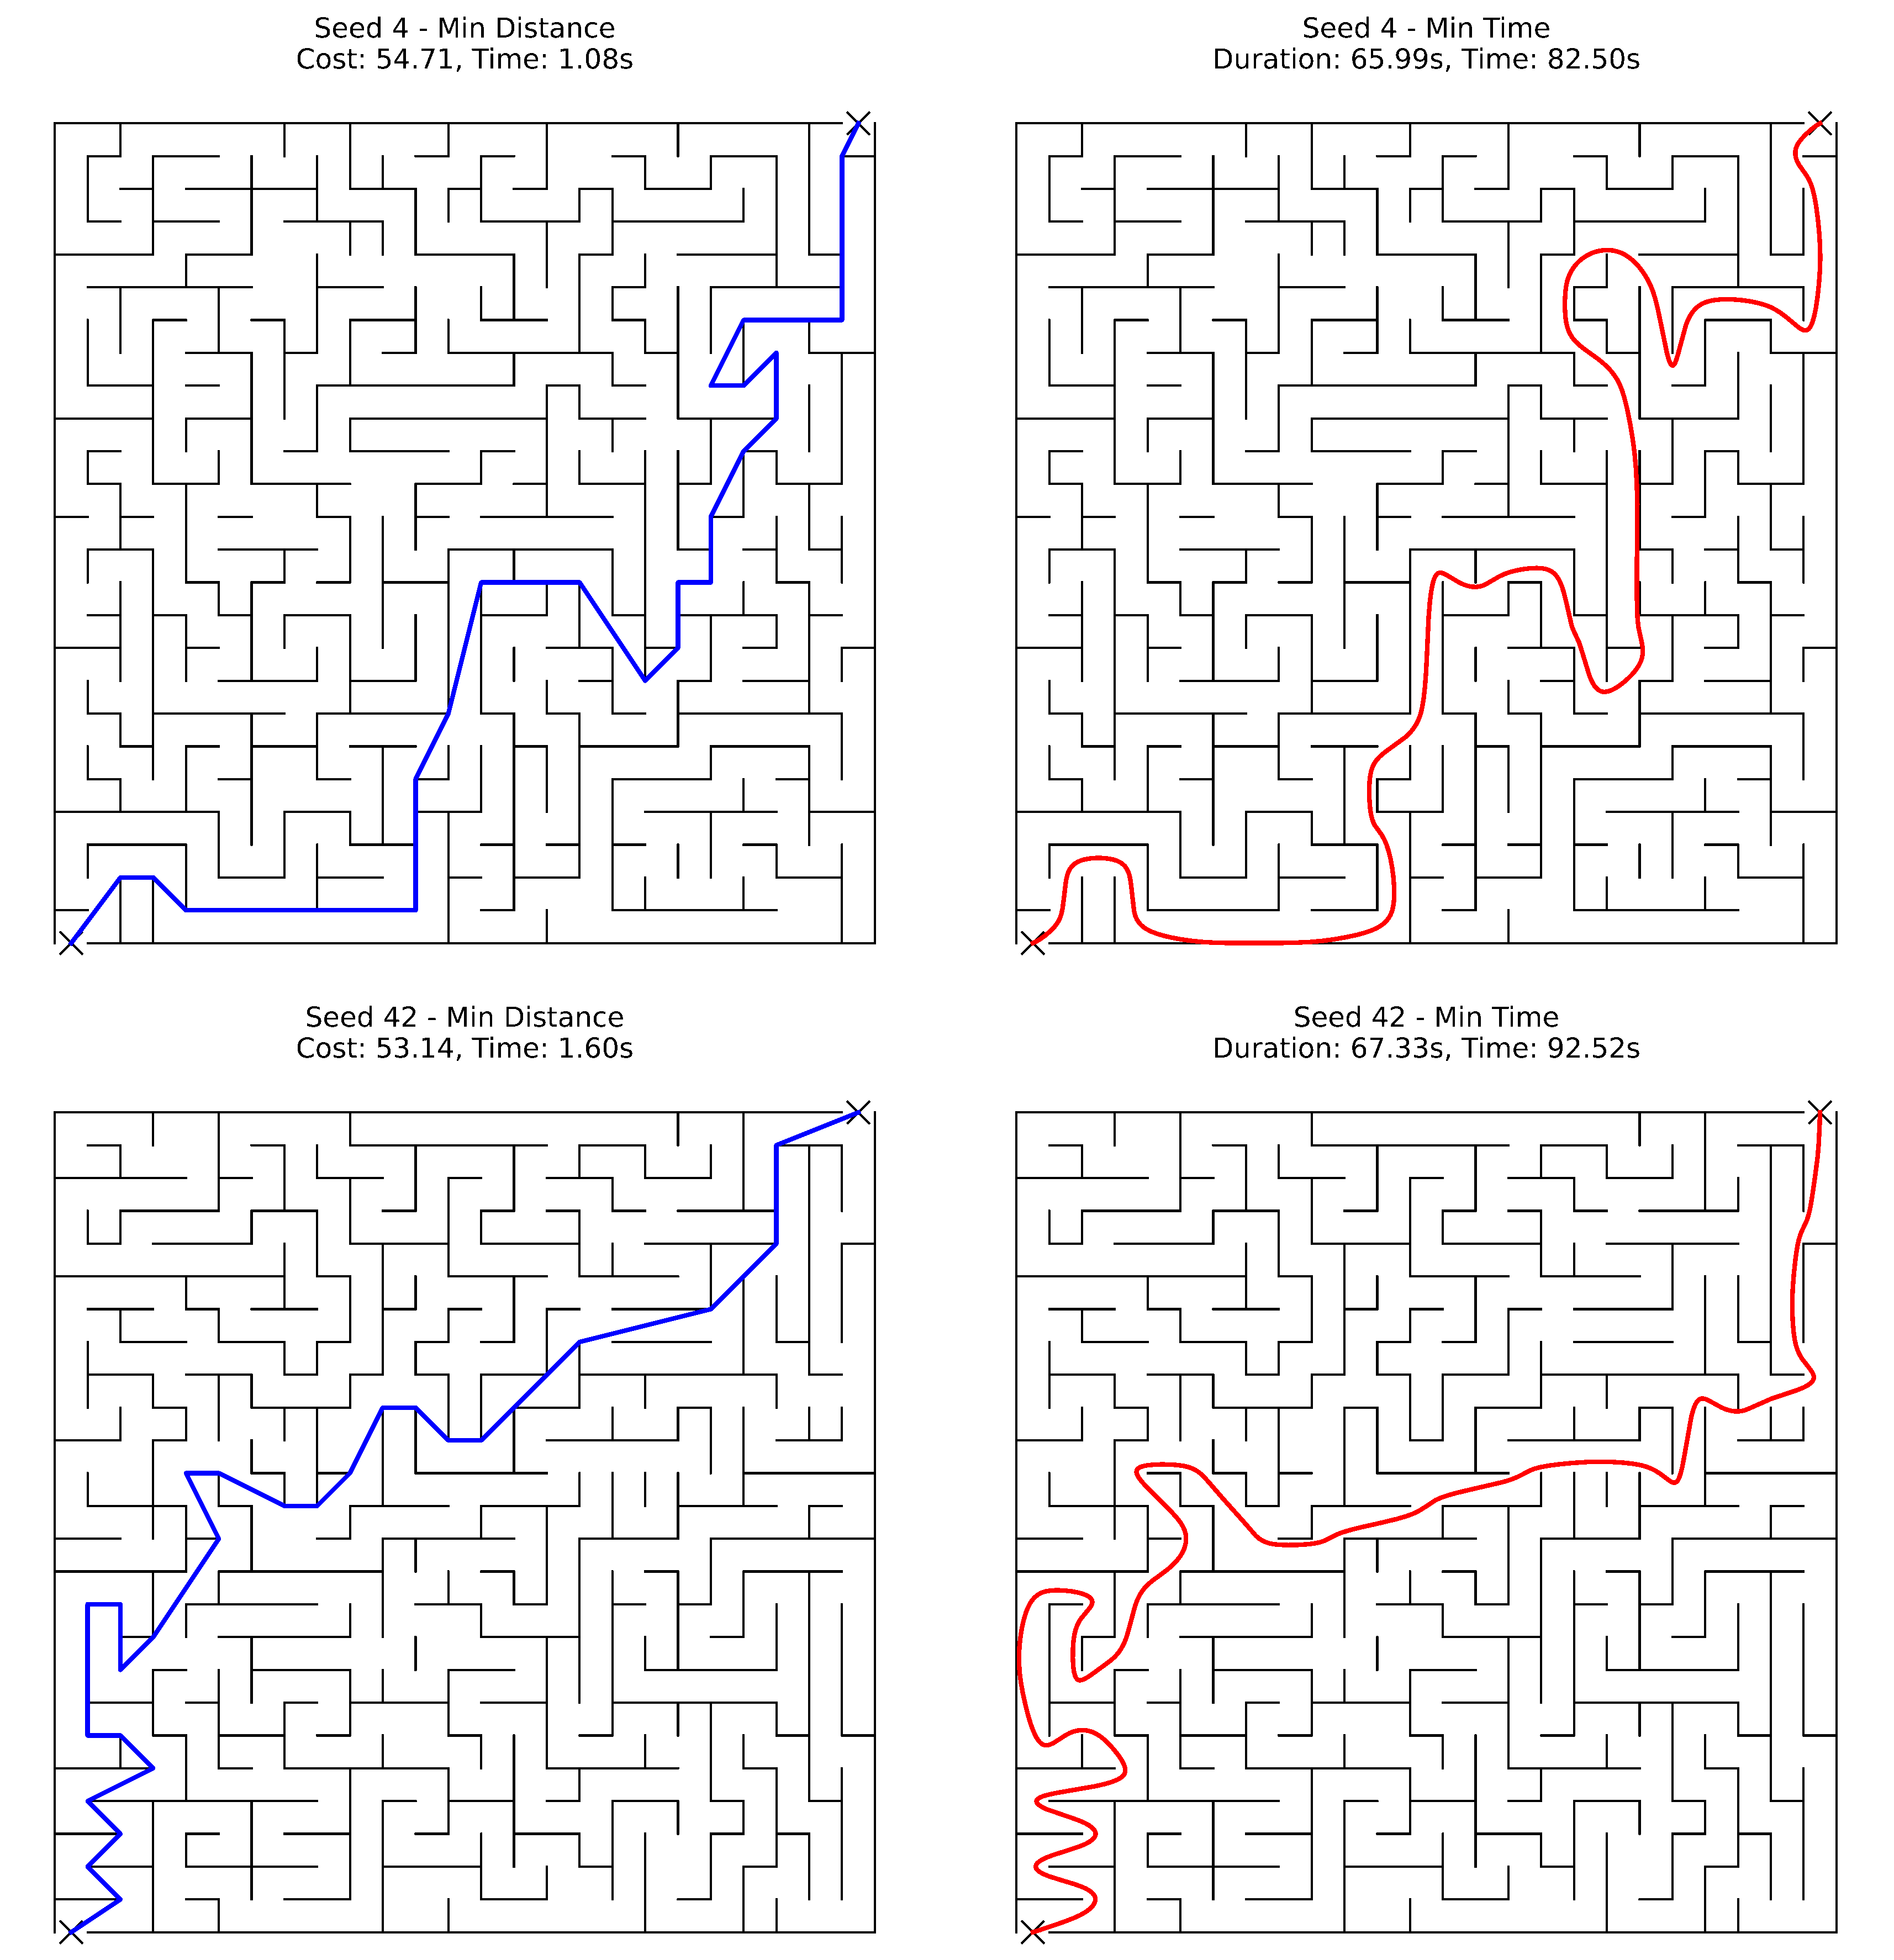
\includegraphics[width=0.7\textwidth]{experiments/image/maze-1.png}
    \caption{Quỹ đạo chuyển động cho 1 số mê cung}
    \label{fig:maze_results}
\end{figure}

\subsubsection{Phân tích Hiệu suất Tính toán và Chi phí Tối ưu}

Dựa trên dữ liệu thu thập từ 10 mẫu thử nghiệm tại bảng \ref{tab:maze_results}, chúng tôi tiến hành so sánh đối chiếu giữa hai phương pháp:
\begin{itemize}
    \item \textbf{Linear GCS}: tối thiểu hóa độ dài hình học.
    \item \textbf{Bézier GCS}: tối thiểu hóa thời gian với ràng buộc động lực học.
\end{itemize}

\begin{table}[!htp]
    \centering
    \caption{Thống kê kết quả thực nghiệm trên 10 mẫu mê cung ngẫu nhiên}
    \label{tab:maze_results}
    \begin{tabular}{|l|c|c|c|}
        \hline
        \textbf{Chỉ số (Metric)} 
        & \textbf{Linear GCS} 
        & \textbf{Bézier GCS} 
        & \textbf{Đơn vị} \\
        \hline
        Thời gian giải trung bình (Mean) 
        & 1,28 
        & 85,22 
        & s \\
        \hline
        Thời gian giải trung vị (Median) 
        & 1,16 
        & 85,10 
        & s \\
        \hline
        Chi phí trung bình (Mean Cost) 
        & 71,88 
        & 88,03 
        & unit \\
        \hline
        Sai số chi phí (Cost Ratio TB) 
        & 0,82 
        & 1,00 
        & x \\
        \hline
    \end{tabular}
\end{table}

Kết quả thống kê cho thấy sự khác biệt rõ rệt về hiệu suất:

\textbf{Về thời gian tính toán}: Linear GCS cho thấy khả năng phản hồi cực nhanh với thời gian giải trung bình chỉ $1,28$ giây. Trong khi đó, Bézier GCS yêu cầu trung bình $85,22$ giây để hội tụ. Sự gia tăng này là do Bézier GCS phải giải quyết các ràng buộc vi phân bậc cao ($C^2$) và tối ưu hóa đồng thời biến thời gian $h$, khiến bài toán SOCP có quy mô lớn hơn đáng kể.
    
\textbf{Về chi phí tối ưu}: Chi phí trung bình của Bézier GCS cao hơn khoảng $22\%$ so với Linear GCS. Tuy nhiên, chi phí của Bézier GCS bao gồm cả thành phần điều chuẩn gia tốc (\textit{Regularization Cost}), phản ánh sự đánh đổi cần thiết để đạt được quỹ đạo mượt mà và khả thi về mặt vật lý.


\subsubsection{Phân tích Đặc điểm Quỹ đạo và Tính Tối ưu Toàn cục}

Quan sát các quỹ đạo tại Hình~\ref{fig:maze_results} (tương ứng với các \textit{Seeds} khác nhau), chúng tôi rút ra các nhận định quan trọng về hành vi của bộ lập kế hoạch:
\begin{enumerate}
    \item \textbf{Sự khác biệt về lộ trình (Homotopy class)}: Trong nhiều trường hợp (ví dụ \textit{Seed 4} và \textit{Seed 42}), quỹ đạo Bézier GCS (màu đỏ) lựa chọn một lộ trình hoàn toàn khác so với quỹ đạo Linear GCS (màu xanh). Trong khi quỹ đạo hình học ưu tiên đường ngắn nhất với nhiều khúc cua gắt, quỹ đạo Bézier chấp nhận đi quãng đường dài hơn nhưng ít góc rẽ gắt hơn nhằm duy trì vận tốc cao và giảm chi phí gia tốc.
    
    \item \textbf{Hành vi tại các góc cua}: Quỹ đạo Bézier thể hiện xu hướng ``ôm cua'' rộng tại các giao lộ để đảm bảo tính liên tục của gia tốc ($C^2$). Các thành phần vận tốc được duy trì trong giới hạn $[-1, 1]$ nhờ vào cấu trúc nón phối cảnh trong mô hình GCS.
    
    \item \textbf{Tính tối ưu toàn cục}: Đối với cả 10 mẫu mê cung, kỹ thuật nới lỏng lồi đều trả về các xác suất nhị phân $\phi_e$ hội tụ về $\{0,1\}$, giúp nghiệm thu được tự động đạt tối ưu toàn cục mà không cần qua bước làm tròn (\textit{Rounding}). Điều này chứng minh GCS vượt trội hơn các phương pháp MICP truyền thống khi giảm số lượng biến nhị phân từ mức $|I|^2$ xuống chỉ còn $2|I|$, cho phép giải quyết các mê cung lớn mà các bộ giải cũ thường thất bại.
\end{enumerate}

Kết luận, việc thực hiện trên 10 mê cung khác nhau đã khẳng định tính ổn định của framework GCS. Mặc dù chi phí tính toán cho quỹ đạo \textit{kinodynamic} cao hơn, GCS cung cấp một giải pháp nhất quán để tìm ra lộ trình trơn tru, an toàn tuyệt đối và tối ưu toàn cục trong các môi trường có độ phức tạp tổ hợp cực cao.


\subsection{Phân tích Thực nghiệm 3: So sánh GCS, RRT và RRT* trên mê cung \texorpdfstring{$25\times 25$}{25x25}}
\label{subsec:rrt_gcs_comparison_results}

Sau khi đánh giá GCS-Bézier trên nhiều mê cung ngẫu nhiên, chúng tôi thực hiện
thêm một thí nghiệm đối chứng trên một mê cung cố định để đặt GCS cạnh các
phương pháp sampling-based quen thuộc.
Mục tiêu của thí nghiệm này không phải là khẳng định một phương pháp luôn vượt
trội trong mọi tiêu chí, mà là làm rõ đánh đổi giữa hai nhóm tiếp cận. GCS khai
thác trực tiếp cấu trúc đồ thị của các vùng lồi để tối ưu đường đi hoặc
quỹ đạo, trong khi RRT/RRT* tìm nghiệm bằng cách mở rộng cây ngẫu nhiên trong
không gian tự do. Vì vậy, các chỉ số như độ dài đường đi, runtime, tỉ lệ thành
công, smoothness được dùng để mô tả các khía cạnh khác nhau của
nghiệm.

\begin{figure}[!htp]
    \centering
    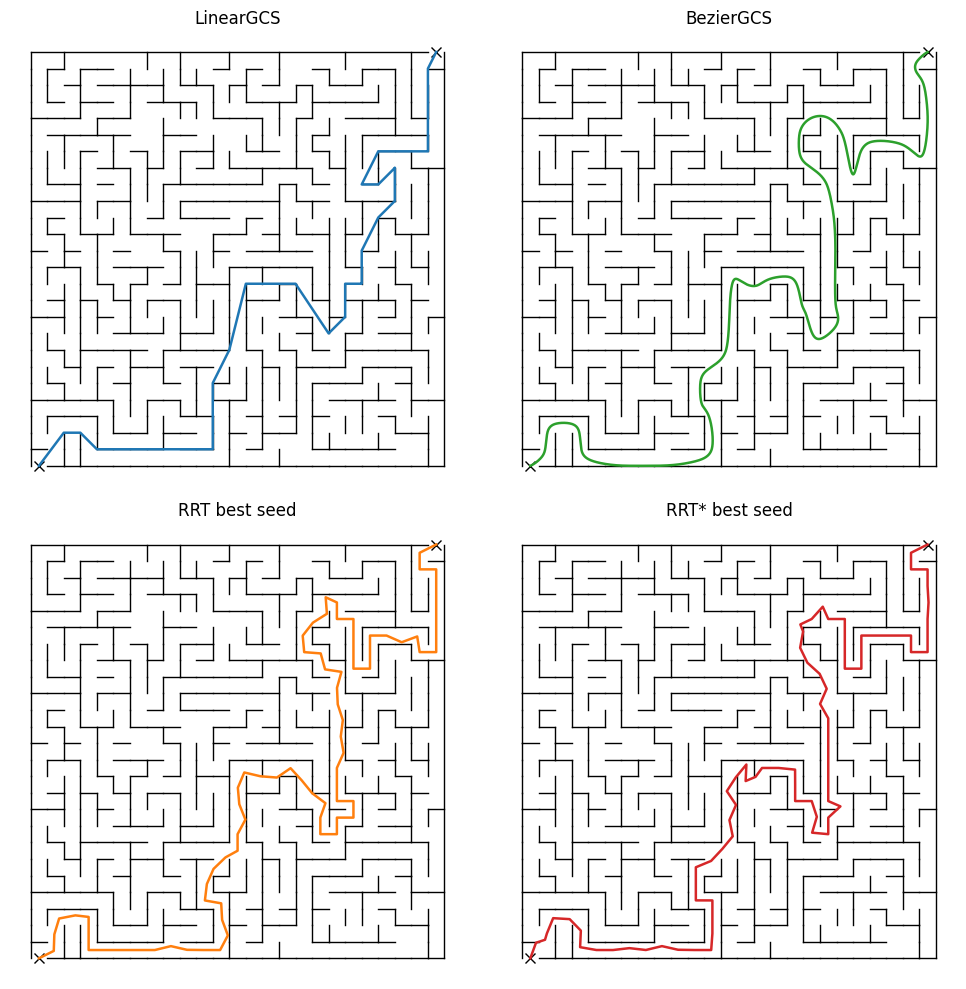
\includegraphics[width=0.7\textwidth]{experiments/image/RRT-GCS/path.png}
    \caption{Các quỹ đạo trên mê cung seed 4 khi so sánh GCS, RRT và RRT* trên cùng một môi trường $25\times 25$.}
    \label{fig:rrt_gcs_paths}
\end{figure}

\begin{figure}[!htp]
    \centering
    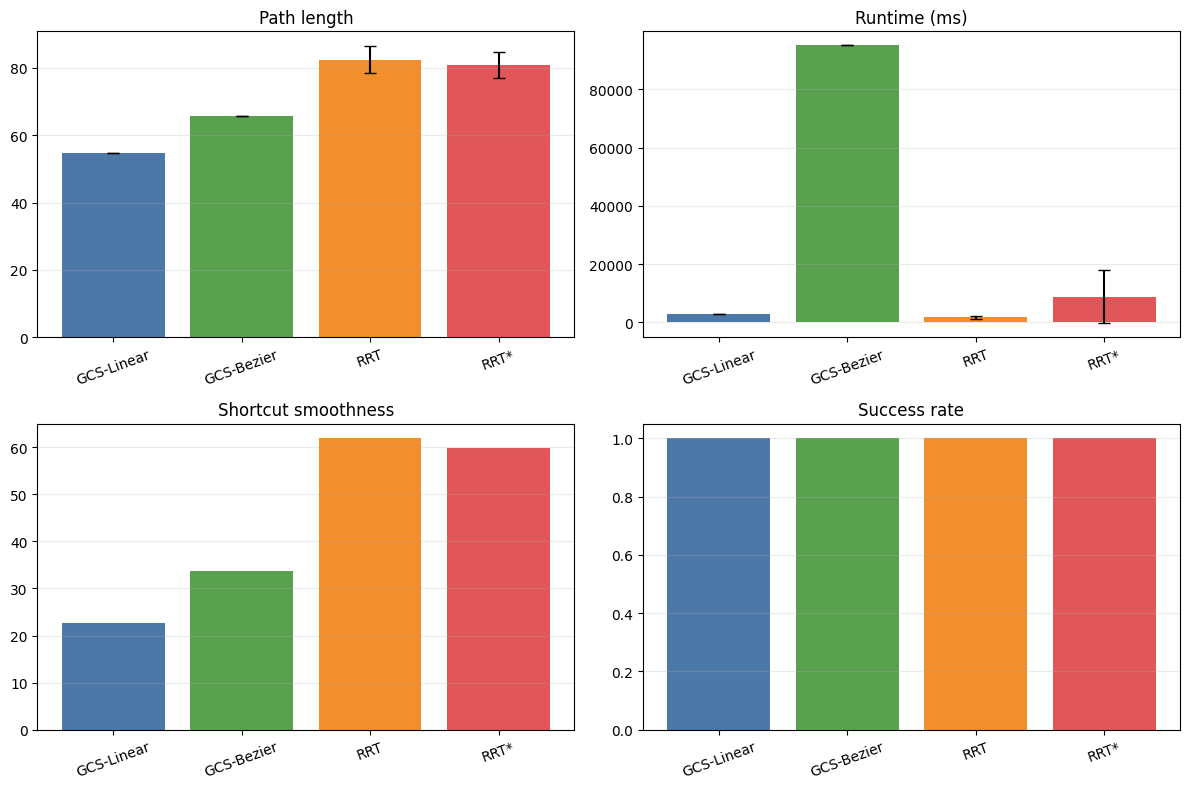
\includegraphics[width=0.9\textwidth]{experiments/image/RRT-GCS/cot.png}
    \caption{So sánh các chỉ số tổng hợp giữa GCS, RRT và RRT* trên mê cung seed 4.}
    \label{fig:rrt_gcs_metrics}
\end{figure}

\begin{table}[!htp]
\centering
\caption{Kết quả định lượng khi so sánh GCS, RRT và RRT* trên mê cung $25\times 25$ seed 4}
\label{tab:rrt_gcs_comparison}
\resizebox{\textwidth}{!}{%
\begin{tabular}{lcccccc}
\toprule
\textbf{Thuật toán}
& \textbf{Độ dài TB}
& \textbf{Độ dài std}
& \textbf{Runtime TB (ms)}
& \textbf{Runtime std (ms)}
& \textbf{Tỉ lệ TC}
& \textbf{Smoothness} \\
\midrule
GCS-Linear
& 54.7117
& 0.0000
& 2847.13
& 0.00
& 1.00

& 22.6444 \\
GCS-Bézier
& 65.8388
& 0.0000
& 95179.93
& 0.00
& 1.00
& 33.6341 \\
RRT
& 82.4245
& 4.0946
& 1715.12
& 432.91
& 1.00
& 61.8902 \\
RRT*
& 80.7592
& 3.8656
& 8790.82
& 9079.57
& 1.00
& 59.9205 \\
\bottomrule
\end{tabular}}
\end{table}

\begin{figure}[!htp]
    \centering
    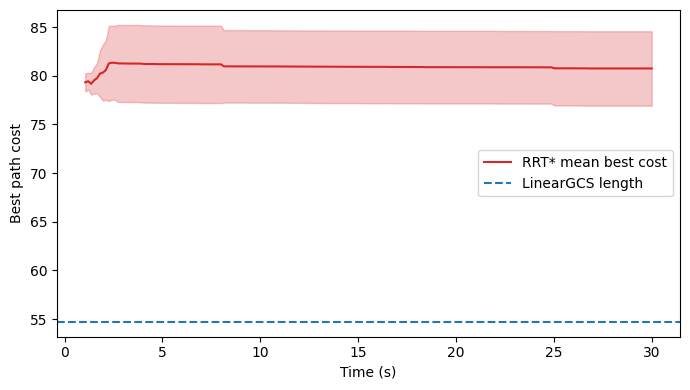
\includegraphics[width=0.78\textwidth]{experiments/image/RRT-GCS/rrt-linear.png}
    \caption{So sánh độ dài đường đi giữa GCS-Linear và các nghiệm sampling-based trên mê cung $25\times 25$ seed 4.}
    \label{fig:rrt_gcs_length_compare}
\end{figure}

\subsubsection{Độ dài đường đi và thời gian chạy}

Bảng~\ref{tab:rrt_gcs_comparison} và Hình~\ref{fig:rrt_gcs_length_compare} cho
thấy GCS-Linear cho đường đi ngắn nhất,
với độ dài trung bình $54.7117$. Kết quả này phù hợp với bản chất của
formulation, vì GCS-Linear tối ưu trực tiếp độ dài hình học trên đồ thị các vùng
lồi. Lấy GCS-Linear làm mốc tham chiếu, GCS-Bézier tạo quỹ đạo dài hơn khoảng
$20.3\%$, RRT dài hơn khoảng $50.7\%$, còn RRT* dài hơn khoảng $47.6\%$. Như
vậy, RRT* có cải thiện so với RRT nhờ cơ chế rewiring, nhưng mức cải thiện trung
bình chỉ khoảng $2.0\%$. Điều này cho thấy với time budget 30 giây và môi trường
nhiều hành lang hẹp, RRT* chưa tiến gần tới chất lượng nghiệm của GCS-Linear.

Xét về runtime, RRT là phương pháp nhanh nhất với thời gian chạy trung bình
khoảng $1.72$ giây. GCS-Linear cần khoảng $2.85$ giây, chậm hơn RRT nhưng vẫn
cùng bậc thời gian và đổi lại cho nghiệm ngắn hơn đáng kể. RRT* đạt nghiệm tốt
nhất được ghi nhận sau trung bình $8.79$ giây, đồng thời có độ lệch chuẩn lớn
($9.08$ giây), phản ánh rõ tính anytime và sự phụ thuộc vào seed lấy mẫu.
GCS-Bézier có runtime lớn nhất, khoảng $95.18$ giây, do bài toán phải xử lý đồng
thời ràng buộc liên tục $C^2$, giới hạn vận tốc, biến co giãn thời gian và các
thành phần điều chuẩn đạo hàm.

\subsubsection{Tỉ lệ thành công, smoothness}

Cả bốn thuật toán đều tìm được nghiệm trong thí nghiệm này. Với GCS-Linear và
GCS-Bézier, nghiệm là deterministic nên các độ lệch chuẩn bằng 0. Với RRT và
RRT*, tỉ lệ thành công được tính trên 50 seed ngẫu nhiên và đều đạt $100\%$,
cho thấy thiết lập sampling và collision checker đủ ổn định đối với mê cung seed
4 trong giới hạn tham số đã chọn.

Chỉ số smoothness trong bảng được tính bằng tổng góc đổi hướng, do đó giá trị
nhỏ hơn tương ứng với đường đi ít gấp khúc hơn theo metric này. GCS-Linear đạt
$22.6444$, GCS-Bézier đạt $33.6341$, RRT* đạt $59.9205$ và RRT đạt $61.8902$.
Hai nghiệm sampling-based vì vậy vẫn kém mượt hơn rõ rệt sau bước shortcut
smoothing. RRT* cải thiện nhẹ so với RRT, nhưng chênh lệch không lớn, phù hợp
với quan sát ở chỉ số độ dài đường đi. Riêng GCS-Bézier cần được diễn giải cẩn
thận: quỹ đạo Bézier có tính trơn theo tham số thời gian và thỏa các ràng
buộc liên tục, nhưng do quỹ đạo có thể dài hơn và được sample dày hơn, tổng góc
đổi hướng tích lũy không nhất thiết nhỏ nhất. Vì vậy, smoothness ở đây hữu ích
để nhận diện độ gấp khúc của RRT/RRT*, nhưng chưa phản ánh đầy đủ chất lượng
động học của quỹ đạo Bézier.

\subsubsection{Nhận xét tổng hợp}

Kết quả trên cho thấy mỗi nhóm phương pháp phù hợp với một mục tiêu sử dụng
khác nhau. Nếu ưu tiên chính là đường đi ngắn, ổn định và có tính deterministic,
GCS-Linear là lựa chọn tốt nhất trong thí nghiệm này. Nếu cần một nghiệm khả thi
nhanh với chi phí tính toán thấp, RRT là baseline hiệu quả, nhưng đổi lại đường
đi dài và gấp khúc hơn đáng kể. RRT* cải thiện chất lượng so với RRT nhờ
rewiring, tuy nhiên mức cải thiện trong mê cung này còn khiêm tốn so với phần
runtime tăng thêm. GCS-Bézier có chi phí tính toán lớn nhất, nhưng cần được xem
như một bài toán khác giàu ràng buộc hơn: phương pháp này tìm quỹ đạo
min-time dưới giới hạn vận tốc và ràng buộc continuity, thay vì chỉ tối thiểu
hóa độ dài hình học.


\subsection{Phân tích Thực nghiệm 4: Môi trường 2D đơn giản và tác động của phân hoạch lồi}

% grid 4 images
\begin{figure}[!htp]
    \centering
    \begin{subfigure}[b]{0.48\textwidth}
        \centering
        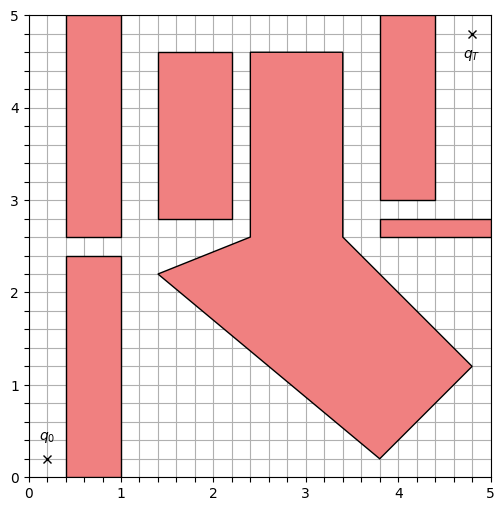
\includegraphics[width=\textwidth]{experiments/image/2d-env.png}
        \caption{Không gian 2D với vật cản (vùng màu đỏ) ban đầu}
        \label{fig:result_a}
    \end{subfigure}
    \hfill
    \begin{subfigure}[b]{0.48\textwidth}
        \centering
        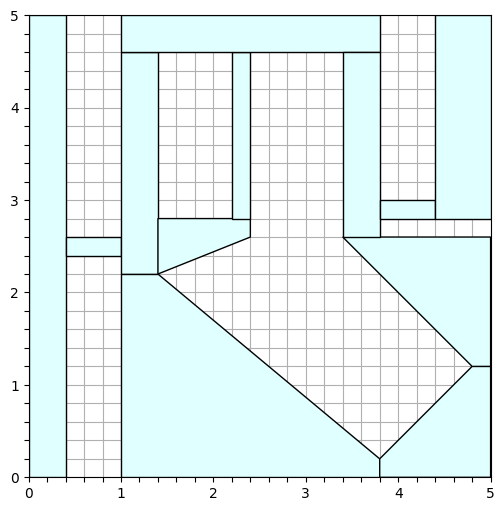
\includegraphics[width=\textwidth]{experiments/image/manual_decompose.png}
        \caption{Kết quả Phân hoạch thủ công}
        \label{fig:result_b}
    \end{subfigure}
    
    \vspace{0.5cm}
    
    \begin{subfigure}[b]{0.48\textwidth}
        \centering
        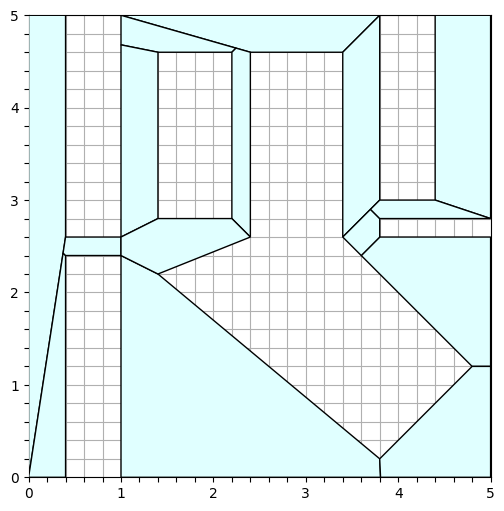
\includegraphics[width=\textwidth]{experiments/image/ACD_decompose.png}
        \caption{Kết quả Phân hoạch ACD}
        \label{fig:result_c}
    \end{subfigure}
    \hfill
    \begin{subfigure}[b]{0.48\textwidth}
        \centering
        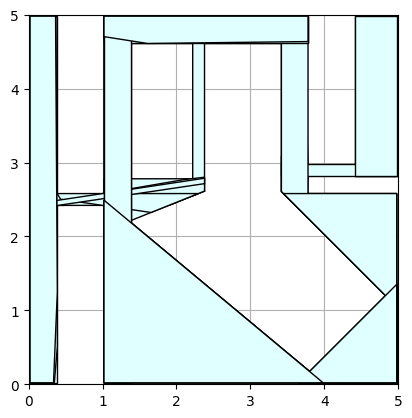
\includegraphics[width=\textwidth]{experiments/image/VCC_decompose.png}
        \caption{Kết quả Phân hoạch VCC}
        \label{fig:result_d}
    \end{subfigure}
    
    \caption[So sánh các phương pháp phân hoạch]{So sánh chất lượng các vùng lồi được phân hoạch bởi các giải thuật khác nhau. Số lượng tập lồi tăng dần từ (b) đến (d), cho thấy sự cải thiện về độ chính xác nhưng tăng độ phức tạp tính toán.}
    \label{fig:results_grid}
\end{figure}


Kết quả thực nghiệm đối với các giải thuật phân hoạch tự động cho thấy sự tương phản rõ rệt về chiến lược biểu diễn không gian cấu hình cũng như chi phí tính toán
giữa hai phương pháp tiếp cận chủ đạo là ACD và VCC. Đối với giải thuật Phân hoạch Lồi Xấp xỉ (ACD), 
kết quả đạt được thể hiện như hình \ref{fig:result_c} ưu thế vượt trội trong môi trường hình học 2D khi chỉ tạo ra 15 vùng lồi, một con số tiệm cận sát với mức tối ưu của phương pháp phân hoạch thủ công là 12 vùng. 
Hiệu suất này được củng cố bởi thời gian xử lý nhanh, chỉ xấp xỉ 0,01 giây, hoàn toàn phù hợp với độ phức tạp lý thuyết $O(nr^2)$ \cite{LienAmato2006} của thuật toán khi xử lý các đa giác có số lượng đỉnh lõm không quá lớn. 
Việc ACD có khả năng kiểm soát mức độ chi tiết thông qua tham số lõm $\tau$ cho phép hệ thống duy trì được sự cân bằng giữa độ chính xác hình học và số lượng vùng lồi tối giản, từ đó giảm thiểu số lượng biến nhị phân trong bài toán quy hoạch nguyên-hỗn hợp (MICP) 
của GCS framework. \\
Ngược lại, giải thuật Visibility Clique Cover (VCC) như được thể hiện thông qua hình \ref{fig:result_d} lại mang đến một cấu trúc phân hoạch dày đặc và phức tạp hơn với số lượng vùng lồi dao động từ 33 đến 35 vùng. Sự thiếu ổn định về số lượng vùng phân hoạch giữa các lần thực thi xuất phát trực tiếp 
từ tính chất ngẫu nhiên của bước lấy mẫu $n$ điểm trong không gian cấu hình tự do $C_{free}$ để xây dựng đồ thị khả kiến đã được nêu ở phần \ref{subsec:vcc}. Mặc dù sự chênh lệch khoảng 1-3 vùng lồi tại các khu vực hành lang hẹp là mức sai số có thể chấp nhận được, nhưng tổng số lượng vùng lồi lớn đã tạo 
ra một gánh nặng tính toán đáng kể cho bộ giải Mosek do số lượng biến nhị phân $y_e$ tăng lên theo tỉ lệ xấp xỉ $2|I|$. Thời gian hội tụ của VCC trong môi trường 2D thực tế không mang lại hiệu quả cao cho các ứng dụng yêu cầu phản hồi tức thời so với các kỹ thuật phân hoạch 
đa giác trực tiếp như ACD. Tuy nhiên, cần phải nhìn nhận rằng VCC được thiết kế như một phương pháp lai ghép mạnh mẽ để xử lý các không gian cấu hình cao chiều, nơi các vật cản không được xác định tường minh bằng các đa giác mà thông qua các bộ kiểm tra va chạm chung. 
Trong các hệ thống có số chiều lớn như cánh tay robot 7 bậc tự do (7-DoF), việc lấy mẫu và tìm lớp phủ clique giúp VCC tự động hóa quá trình đặt các điểm mầm chiến lược cho thuật toán IRIS, điều mà các phương pháp phân hoạch hình học 2D đơn giản không thể thực hiện được. 
Do đó, việc áp dụng VCC vào môi trường 2D trong thực nghiệm này chủ yếu đóng vai trò kiểm chứng khả năng bao phủ toàn cục và tính an toàn của quỹ đạo.

% filepath: /home/dang-khoa/university/Capstone Project/Report Source/experiments/resutls.tex
\subsubsection{Đánh giá ảnh hưởng của kết quả phân hoạch đến GCS-Bézier}
% Grid 3 ảnh (2 ảnh trên, 1 ảnh dưới giữa)
\begin{figure}[!htp]
    \centering
    \begin{subfigure}[b]{0.48\textwidth}
        \centering
        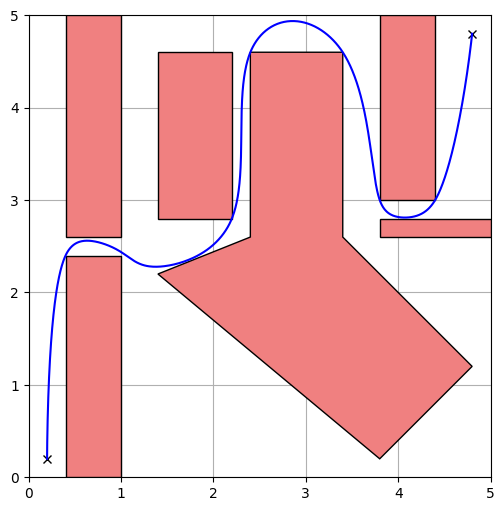
\includegraphics[width=\textwidth]{experiments/image/manual_traj.png}
        \caption{Quỹ đạo chuyển động với phân hoạch thủ công}
        \label{fig:result_manual}
    \end{subfigure}
    \hfill
    \begin{subfigure}[b]{0.48\textwidth}
        \centering
        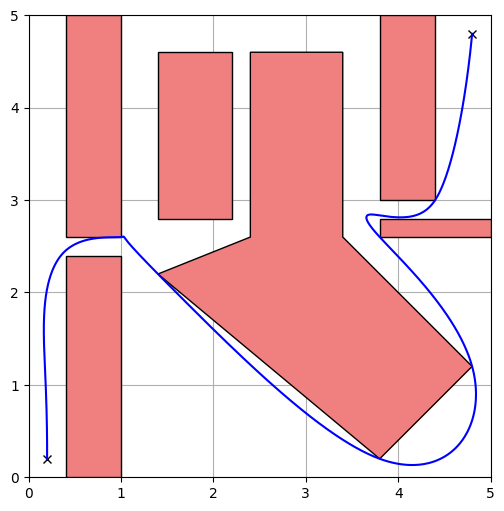
\includegraphics[width=\textwidth]{experiments/image/ACD_traj.png}
        \caption{Quỹ đạo chuyển động với phân hoạch ACD}
        \label{fig:result_acd}
    \end{subfigure}
    
    \vspace{0.5cm}
    
    \begin{subfigure}[b]{0.48\textwidth}
        \centering
        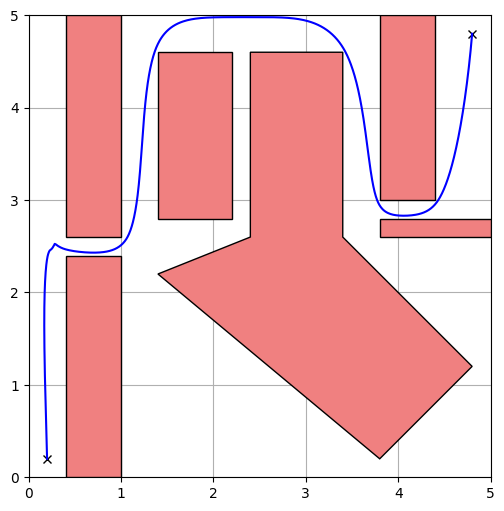
\includegraphics[width=\textwidth]{experiments/image/VCC_traj.png}
        \caption{Quỹ đạo chuyển động với phân hoạch VCC}
        \label{fig:result_vcc}
    \end{subfigure}
    
    \caption[So sánh các quỹ đạo chuyển động cho từng phương pháp phân hoạch]{So sánh chất lượng các quỹ đạo được hoạch định cho tập các vùng lồi được tạo bởi các giải thuật ở trên.}
    \label{fig:results_grid_3}
\end{figure}


\begin{table}[htbp]
\centering
\caption{So sánh hiệu năng giữa các phương pháp lập kế hoạch quỹ đạo}
\label{tab:comparison_all}
\resizebox{\textwidth}{!}{%
\begin{tabular}{lcccccc}
\toprule
\textbf{Phương pháp} 
& \textbf{Thời gian phân hoạch (s)} 
& \textbf{Số vùng} 
& \textbf{Thời gian giải (s)} 
& \textbf{Time cost (s)} 
& \textbf{Path cost (rounded)} 
& \textbf{Tổng thời gian (s)} \\
\midrule
VCC       
& 5.7807 
& 33 
& 269.9363 
& 13.2217 
& 24.4365 
& 275.7170 \\
ACD             
& 0.0109 
& 15 
& 4.3105   
& 12.7875 
& 24.6286 
& 4.3214 \\
Phân hoạch thủ công 
& --     
& 12 
& 3.9005   
& 13.3565 
& 27.8805 
& 3.9005 \\
\bottomrule
\end{tabular}}
\end{table}



Sau khi hoàn tất giai đoạn phân hoạch không gian tự do thành các tập hợp vùng lồi, chúng tôi tiến hành thực hiện bài toán hoạch định quỹ đạo dựa trên khung làm việc Đồ thị các Tập lồi (GCS-Bézier). Mục tiêu của giai đoạn này là tìm kiếm một lộ trình tối ưu không chỉ về mặt hình học mà còn phải đáp ứng các ràng buộc về động lực học và độ trơn của quỹ đạo. Để đạt được sự cân bằng giữa thời gian thực thi vật lý ($T_{duration}$) và nỗ lực điều khiển (Control effort), hàm mục tiêu tổng hợp (Rounded Cost) được thiết lập như sau:
$$Rounded Cost \approx (1 \times T_{duration}) + \sum \left( 0.1 \times \int_{0}^{T_e} \|\text{a}(t)\|^2 dt \right)$$

Trong đó, trọng số cho thời gian thực thi được đặt là $w_{t}=1$ và hệ số điều chuẩn đạo hàm bậc hai (gia tốc) là $\epsilon = 0.1$ nhằm giảm thiểu hiện tượng rung động (jerk) khi robot di chuyển qua các ranh giới vùng lồi. Các kết quả định lượng về hiệu suất tính toán và chất lượng quỹ đạo được phân tích chi tiết dựa trên dữ liệu thu được từ bộ giải Mosek.

\subsubsection*{Hiệu suất tính toán và Khả năng đáp ứng thời gian thực}

Kết quả thực nghiệm tại bảng \ref{tab:comparison_all} cho thấy một sự tương quan phi tuyến tính chặt chẽ giữa số lượng vùng lồi được phân hoạch và thời gian hội tụ của bộ giải. Phương pháp \textbf{VCC} cho thấy hiệu năng kém nhất trong môi trường thực nghiệm 2D. Mặc dù số lượng vùng lồi được tạo ra (33 vùng) chỉ cao hơn gấp đôi so với ACD, nhưng thời gian giải bài toán tối ưu hóa lại rất lớn lên tới xấp xỉ 269,94 giây. Hiện tượng này xuất phát từ việc gia tăng số lượng vùng lồi dẫn đến sự bùng nổ của các biến quyết định nhị phân  và các ràng buộc nón phối cảnh liên kết, khiến không gian tìm kiếm tổ hợp vượt quá khả năng xử lý hiệu quả của bộ giải trong thời gian thực.

Ngược lại, phương pháp \textbf{ACD} thể hiện tính thực tiễn vượt trội khi tổng thời gian thực thi (bao gồm cả phân hoạch và giải quỹ đạo) chỉ mất 4,32 giây, nhanh gấp khoảng 64 lần so với VCC. Kết quả này khẳng định rằng đối với các ứng dụng di động trong môi trường 2D, một cấu trúc phân hoạch tối giản (15 vùng) là yếu tố tiên quyết để duy trì khả năng phản hồi nhanh của hệ thống. Trong khi đó, phương pháp \textbf{Phân hoạch thủ công} mặc dù đạt thời gian giải nhanh nhất (3,90 giây) do cấu trúc đồ thị đơn giản (12 vùng), nhưng không được xem là giải pháp khả thi cho các hệ thống tự hành do đòi hỏi sự can thiệp trực tiếp từ con người, vốn là một rào cản lớn đối với tính tự chủ của robot.

\subsubsection*{Chất lượng Quỹ đạo và Sự đánh đổi giữa các Mục tiêu Tối ưu}

Chất lượng của quỹ đạo được đánh giá thông qua sự đánh đổi giữa thời gian di chuyển thực tế và giá trị tối ưu của hàm mục tiêu (Path cost).

\textbf{Phương pháp VCC}: Đạt giá trị Path cost thấp nhất ($24,44$), đại diện cho nghiệm tối ưu nhất về mặt toán học. Việc chia nhỏ không gian thành nhiều vùng lồi diện tích nhỏ cho phép bộ giải có nhiều "không gian tự do" hơn để tinh chỉnh đường cong Bézier, từ đó tối ưu hóa nỗ lực điều khiển và giảm thiểu tối đa các pha phạt gia tốc. Tuy nhiên, thời gian thực thi vật lý ($13,22$ giây) lại chậm hơn ACD, cho thấy hệ thống chấp nhận di chuyển với vận tốc thấp hơn để đổi lấy độ trơn tuyệt đối. \\
\textbf{Phương pháp ACD}: Mang lại kết quả thực dụng nhất khi robot hoàn thành nhiệm vụ với thời gian ngắn nhất ($12,79$ giây). Mặc dù Path cost ($24,63$) cao hơn nhẹ so với VCC, nhưng sự chênh lệch này không đáng kể trong vận hành thực tế. Điều này chứng tỏ ACD đã tạo ra một quỹ đạo "thực dụng": chạy nhanh, đủ mượt mà và duy trì được tính toán hiệu quả. \\
\textbf{Phân hoạch thủ công}: Thể hiện hiệu năng kém nhất về mặt chất lượng quỹ đạo với Path cost cao nhất ($27,88$) và thời gian di chuyển lâu nhất ($13,36$ giây). Nguyên nhân chủ yếu nằm ở việc phân chia vùng dựa trên trực giác con người thường tạo ra các vùng lồi thô, các vùng có thể to nhưng hình dạng không tối ưu cho robot lách qua, hoặc các điểm nối giữa các vùng bị đặt ở vị trí xấu, khiến robot phải đi đường vòng hoặc phanh gấp tại các giao điểm.


\subsubsection{Đánh giá ảnh hưởng của kết quả phân hoạch đến GCS-DMS}

Bên cạnh nghiệm GCS-Bézier, chúng tôi tiếp tục giải cùng môi trường 2D bằng GCS-DMS để đánh giá tác động của phân hoạch lồi khi quỹ đạo phải thỏa mãn trực tiếp động lực học phi tuyến của mô hình Unicycle. Khác với GCS-Bézier, nghiệm GCS-DMS không chỉ là một đường cong hình học trong mặt phẳng mà còn bao gồm trạng thái, thời lượng từng đoạn và các biến điều khiển nội tại của bài toán multiple shooting. Vì vậy, các giá trị cost trong phần này được dùng để so sánh nội bộ giữa các phân hoạch của GCS-DMS, không được diễn giải như cùng một đại lượng với Path cost của GCS-Bézier.

\begin{figure}[!htp]
    \centering
    \begin{subfigure}[b]{0.48\textwidth}
        \centering
        
\includegraphics[width=\textwidth]{experiments/image/dms/2d_dms_manual.png}
        \caption{GCS-DMS với phân hoạch thủ công}
        \label{fig:dms_2d_manual}
    \end{subfigure}
    \hfill
    \begin{subfigure}[b]{0.48\textwidth}
        \centering
        
\includegraphics[width=\textwidth]{experiments/image/dms/2d_dms_acd.png}
        \caption{GCS-DMS với phân hoạch ACD}
        \label{fig:dms_2d_acd}
    \end{subfigure}
    
    \vspace{0.5cm}
    
    \begin{subfigure}[b]{0.48\textwidth}
        \centering
        
\includegraphics[width=\textwidth]{experiments/image/dms/2d_dms_vcc.png}
        \caption{GCS-DMS với phân hoạch VCC}
        \label{fig:dms_2d_vcc}
    \end{subfigure}
    
    \caption{Quỹ đạo GCS-DMS trên môi trường 2D đơn giản với ba phương pháp phân hoạch khác nhau. Vùng màu xanh nhạt là các vùng được kích hoạt trên đường đi; đường cong màu xanh thể hiện quỹ đạo liên tục sau khi giải bài toán multiple shooting.}
    \label{fig:dms_2d_decomp_compare}
\end{figure}

\begin{table}[!htp]
\centering
\caption{Kết quả GCS-DMS trên môi trường 2D với các phân hoạch khác nhau}
\label{tab:dms_2d_decomp_results}
\resizebox{\textwidth}{!}{%
\begin{tabular}{lcccccccc}
\toprule
\textbf{Phân hoạch}
& \textbf{Số vùng}
& \textbf{Vùng kích hoạt}
& \textbf{Duration (s)}
& \textbf{Thời gian giải (s)}
& \textbf{Cost}
& \textbf{Defect}
& \textbf{Connection gap}
& \textbf{Violation} \\
\midrule
Thủ công
& 12
& 7
& 23.15
& 17.38
& 47.35
& $0.00$
& $8.98\times 10^{-9}$
& $8.78\times 10^{-9}$ \\
ACD
& 15
& 9
& 25.47
& 34.23
& 51.55
& $2.07\times 10^{-14}$
& $4.87\times 10^{-9}$
& $1.10\times 10^{-8}$ \\
VCC
& 33
& 7
& 20.91
& 26.36
& 76.26
& $0.00$
& $6.11\times 10^{-11}$
& $9.73\times 10^{-9}$ \\
\bottomrule
\end{tabular}}
\end{table}

Kết quả tại Bảng~\ref{tab:dms_2d_decomp_results} cho thấy cả ba phân hoạch đều cho nghiệm khả thi về mặt số học: defect dynamics gần bằng không, connection gap nhỏ hơn $10^{-8}$ và mức vi phạm ràng buộc hình học cũng ở mức $10^{-8}$. Điều này xác nhận rằng pipeline GCS-DMS có thể phục hồi quỹ đạo động lực liên tục từ các phân hoạch có cấu trúc khá khác nhau.

Xét riêng chất lượng nghiệm, phân hoạch thủ công đạt cost thấp nhất ($47.35$) và thời gian giải ngắn nhất ($17.38$ giây), chủ yếu nhờ số vùng ít và chuỗi vùng kích hoạt ngắn. ACD tạo ra nghiệm có cost gần với phân hoạch thủ công ($51.55$), nhưng thời gian giải cao hơn do đường đi đi qua nhiều vùng hơn. VCC cho thời gian thực thi quỹ đạo ngắn nhất ($20.91$ giây), tuy nhiên cost lớn nhất ($76.26$), phản ánh việc nghiệm phải đánh đổi thêm nỗ lực điều khiển và cấu trúc chuyển tiếp phức tạp giữa các vùng nhỏ. Đáng chú ý, dù VCC tạo ra nhiều vùng nhất, đường đi cuối cùng chỉ kích hoạt 7 vùng; điều này cho thấy số vùng toàn cục không phải yếu tố duy nhất quyết định chất lượng nghiệm DMS, mà hình học của các vùng được chọn và vị trí giao giữa chúng cũng đóng vai trò quan trọng.

Tóm lại, thông qua các chỉ số đo lường thực nghiệm, \textbf{ACD} vẫn là lựa chọn cân bằng nhất cho môi trường 2D đơn giản khi xét đồng thời hai formulation: với GCS-Bézier, ACD cho thời gian giải rất thấp và chất lượng quỹ đạo gần với VCC; với GCS-DMS, ACD cho nghiệm khả thi có cost gần phân hoạch thủ công trong khi vẫn giữ được tính tự động của quá trình phân hoạch. Phân hoạch thủ công có lợi thế về độ gọn của đồ thị nhưng không phù hợp với hệ thống tự hành, còn VCC phù hợp hơn như một cơ chế bao phủ tổng quát cho các không gian cấu hình phức tạp hoặc các bài toán ngoại tuyến.
